%----------------------------------------------------------------------------------------
%       CHAPTER 10
%----------------------------------------------------------------------------------------

\cleardoublepage

\chapterimage{origin.jpg} % Chapter heading image

\chapter{The geological cycle of carbon}\label{ch:geological-carbon}

\hfill \break

\vspace{24mm}

\noindent

%------------------------------------------------
\newpage
%------------------------------------------------

\section*{README}

Download the following \textit{re-start} files:

\vspace{2mm}
\begin{itemize}[noitemsep]
\vspace{1mm}
\item [] Modern (8-level) marien carbon cycle state [\textit{Ridgwell and Hargreaves}, 2007]:
\vspace{-1mm}\small\begin{verbatim}
$ wget --no-check-certificate http://www.seao2.info/cgenie_output/
   cookie.CBSR.p_worbe2.BASES.RidgwellHargreaves.SPIN2.tar.gz
\end{verbatim}\normalsize\vspace{-1mm}
\vspace{1mm}
\item [] Idealized continental configuration following \textit{Hulse and Ridgwell} [2025]:
\vspace{-1mm}\small\begin{verbatim}
wget --no-check-certificate http://www.seao2.info/cgenie_output/
   cookie.CBSR.fkl_pp51.BASESw.DSEA1MUDS2REEF0_10_00.pNOSEAS.SPIN1
\end{verbatim}\normalsize\vspace{-1mm}
\end{itemize}

\vspace{1mm}
\noindent and then extract:

\vspace{2mm}
\begin{itemize}[noitemsep]
\vspace{1mm}
\item [] \vspace{-0mm}\small\begin{verbatim}
$ tar xfzv cookie.CBSR.p_worbe2.BASES.RidgwellHargreaves.SPIN2.tar.gz
\end{verbatim}\normalsize\vspace{-0mm}
\vspace{1mm}
\item [] \vspace{-0mm}\small\begin{verbatim}
$ tar xfzv cookie.CBSR.fkl_pp51.BASESw.DSEA1MUDS2REEF0_10_00.pNOSEAS.SPIN1
\end{verbatim}\normalsize\vspace{-0mm}
\end{itemize}


%------------------------------------------------
\newpage
%------------------------------------------------

\section*{The long tail of CO$_{2}$ (and other tales from the sediments)}

This chapter introduces the marine sediment and terrestrial weathering modules in \textbf{cookie}. In terms of the fate of fossil fuel \(CO_{2}\), the model configuration and experiments in this chapter include: a representation of deep-sea sediments and the interaction between the preservation and burial of \(CaCO_{3}\) and ocean chemistry plus, plus the balance (or imbalance) between weathering on land and sedimentary burial (of \(CaCO_{3}\)) (all in addition to the interaction between atmosphere and ocean and redistribution of carbon within the ocean as previously). For an over-view of the sediment model and what time-scales and nature of carbon cycle interaction between ocean and sediment you can expect, read: \textit{Ridgwell and Zeebe} [2005] and \textit{Ridgwell and Hargreaves} [2007]. \textbf{ROKGEM} is described in \textit{Colbourn et al.} [2013].

Beyond the basic 'inorganic' geological carbon cycle\footnote{As per described in the references above.}, other geological cycles, ocean-sediment and atmosphere-rock interactions\footnote{All these processes and feedbacks can be 'fixed' (made invariant) or disabled to test their importance (or not) in the long-term regulation of atmospheric \(pCO_{2}\) and climate dynamics and in comparison with published analyses based only on the 'inorganic' carbon cycle (and silicate weathering as the only long-term feedback on atmospheric \(pCO_{2}\)).}  that can be accounted for in the model and explored in this Chapter are:

\vspace{1mm}
\begin{itemize}[noitemsep]
\setlength{\itemindent}{.2in}
\item Weathering of rock-hosted organic carbon (kerogens).
\item Weathering of phosphorous (e.g. from apatite).
\item Burial of organic carbon (as a function of the organic matter deposition flux to the sediment surface).
\item Differential regeneration and return of dissolved phosphorous back to the ocean (creating a strong nonlinear feedback with the dissolved oxygen concentration in the ocean interior).
\end{itemize}

\begin{figure}
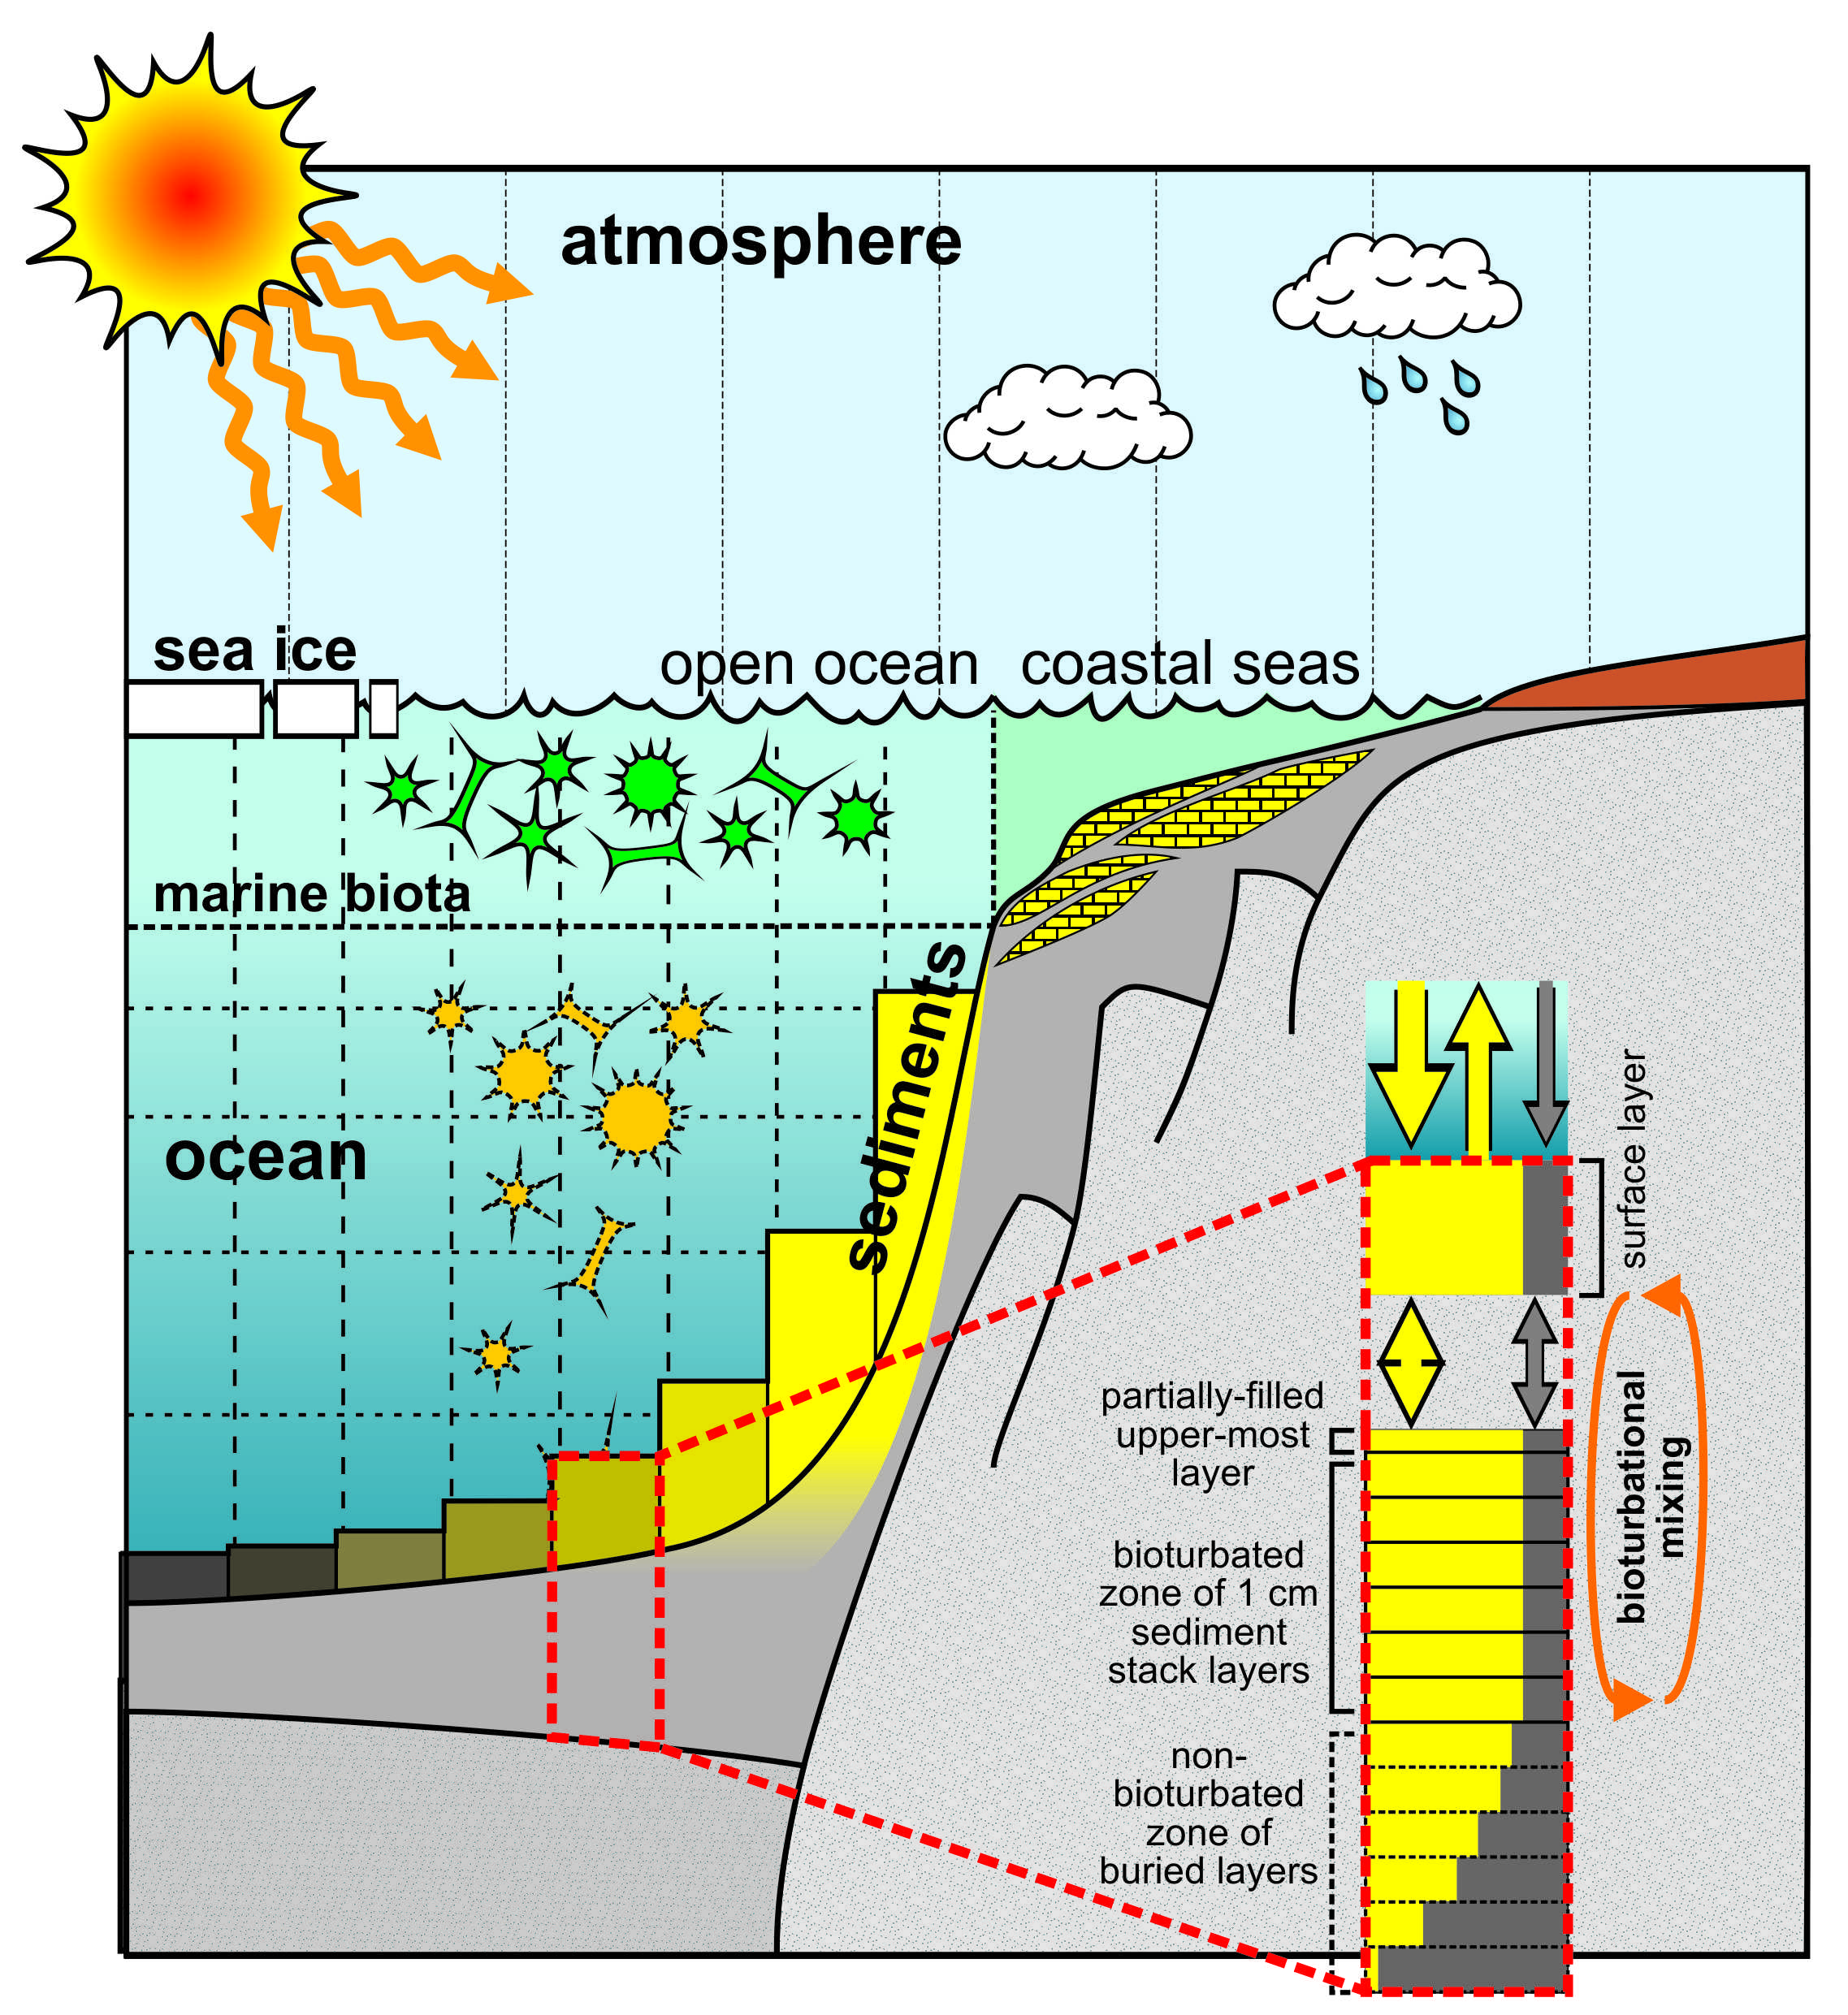
\includegraphics[width=0.5\textwidth]{sediments.jpg}
\caption{Schematic of \textbf{SEDGEM} sediment component.}
\label{fig:sediments}
\end{figure}

%------------------------------------------------
\vspace{1mm}\noindent\rule{4cm}{0.1mm}\vspace{2mm}
%------------------------------------------------

%------------------------------------------------
\newpage
%------------------------------------------------

\section{Sediment model output}

This configuration of \textbf{cookie} generates additional \textit{time-series} output of sediment properties: \textsf{\footnotesize timeseries\_sed\_seafloor\_*.txt}. For example, \textsf{\footnotesize timeseries\_sed\_seafloor\_CaCO3.txt} records how the mean \(CaCO_{3}\) content of surface sediments (uppermost sediment layer) evolves with time. There are also \textit{time-series} file outputs that record the evolution of burial (and dissolution) fluxes as well as weathering -- all of which will be important for fully understanding system behavior\footnote{In the default output, only key sources and sinks are saved -- \textsf{\footnotesize timeseries\_geo\_*.txt}.}. As per with the ocean (-atmosphere) data saving, a summary file of sediment fluxes and composition is also saved -- \textsf{\footnotesize INFO\_sediment\_summary\_AT\_END.txt}, but now only at the very end of the experiment and not tied to the saving of each \textit{time-slice}). In addition, there is a parameter value summary for use in configuring weathering (discussed later) -- \textsf{\footnotesize INFO\_weathering\_parameters\_AT\_END.txt} 

%------------------------------------------------
\vspace{1mm}\noindent\rule{4cm}{0.1mm}\vspace{2mm}
%------------------------------------------------

\noindent 2D (e.g. surface sediment properties, fluxes, etc.) output is saved in the \textsf{\footnotesize results} sub-directory of your experiment directory in a \textbf{netCDF} file called \textsf{\footnotesize fields\_sediments\_2d.nc}. For example, the 2D distribution of \(wt\% CaCO_{3}\) –- which is the weight fraction of calcium carbonate (\(CaCO_{3}\)) in the surface sediments of the deep ocean (i.e., how much plankton carbonate shell material is there compared to other stuff in the mud at the bottom of the ocean) -- is saved here\footnote{In a variable called: \textsf{\footnotesize sed\_CaCO3}}. 

\vspace{1mm}
\noindent \textbf{Note}: The saving of spatial, \textbf{netCDF} output for the sediments, only occurs \uline{at the very end} of a model experiment. However, there is some duplication of results saving, and \textit{time-slices} of sediment composition are also saved in: \textsf{\footnotesize fields\_ocean\_2d.nc}.

%------------------------------------------------
\vspace{1mm}\noindent\rule{4cm}{0.1mm}\vspace{2mm}
%------------------------------------------------

\subsection{Simulating the marine geological record ('\textit{sedcores}')}

\textbf{cookie} generates sediment records -- ‘\textit{sedcores}’ (e.g. see: \textit{Ridgwell} [2007]) -- and hence simulates what one might expect to see in a marine sediment core recovered from the ocean floor. The locations of these cores are either stored in a file listing their locations\footnote{Parameter: \textsf{sg\_par\_sedcore\_save\_list\_name}} or in an ASCII ‘map’ of the ocean, whose filename is given by the parameter: \texttt{\small sg\_par\_sedcore\_save\_mask\_name}. Simply by flipping a '\texttt{\small 0.0}' to a '\texttt{\small 1.0}', \textbf{cookie} will generate and save a sediment ‘core’ at that particular (\textit{i,j}) location. For example, in the folder: \textsf{\footnotesize genie-paleo/p\_worjh2}, the file \textsf{\footnotesize worjh2\_save\_mask.36x36} contains 5 '\texttt{\small 1}s' clustered in the Eastern Mediterranean basin.\footnote{\textbf{cookie} does not distinguish between a '\texttt{\small 00}' and a '\texttt{\small 0}' -- this is simply to help you orientate yourself and identify land ('\texttt{\small 00}') vs. ocean with no sedcore defined ('\texttt{\small 0}').}

%------------------------------------------------
\vspace{1mm}\noindent\rule{4cm}{0.1mm}\vspace{2mm}
%------------------------------------------------

\noindent Sediment \textit{cores} are saved in the \textsf{\footnotesize results} sub-directory of your experiment directory in a \textbf{netCDF} file called \textsf{\footnotesize fields\_sediments\_1d.nc}. Individual sediment \textit{cores} are assigned an integer starting at $1$, with the spatial pattern of IDs saved in \textsf{\footnotesize fields\_sediments\_2d.nc} as variable \textsf{\footnotesize grid\_ID\_sedcore}. In \textsf{\footnotesize fields\_sediments\_1d.nc}, these IDs form the \textit{x}-axis for all the saved variable fields, with accumulated sediment depth as the \textit{y}-axis.

\textbf{Note}: You may need to switch the \textbf{Panoply} file contents display settings at the bottom from \textsf{\footnotesize Show: Georeferenced variables} to \textsf{\footnotesize Show: Plottable variables} (or \textsf{\footnotesize Show: All variables}) because the \textit{x}-axis is not a spatial dimension (such as latitude).

%------------------------------------------------
\newpage
%------------------------------------------------

Sediment \textit{cores} reflect not only the material which has accumulated (or not accumulated, or accumulated but  subsequently dissolved …) during the course of your experiment, but also the material that has accumulated during any \textit{re-start} ... \uline{plus}, whatever material the sediment \textit{core} was initialized with to start with. For example, the large interval of initially 100\% detrital material at the base of the sediment core simply reflects the initialization of the sediment array in the model. Also note the ash ‘peak’ near the bottom of the stack (filled) sediment layers – this is a tracer to ‘tag’ the start of the model spin-up. If you look at the spin-up results -– the ash peak lies in a sediment layer with age equal to the total length of of the spin-up carried out.\footnote{\textbf{Q.} Why is there any ash deeper than the age corresponding to the start of the spin-up? How can it get there (i.e. what processes could move solid material deeper within the sediment column)?} Saved variables include:

\vspace{1mm}
\begin{itemize}[noitemsep]
\item \textsf{\footnotesize phys\_layer } –- sediment layer number (counting down).
\item \textsf{\footnotesize phys\_depth } -– (cumulative) depth below surface, measured from the sediment surface to the mid-point of each sediment layer (cm).
\item \textsf{\footnotesize th (cm) } -- thickness of each sediment layer (cm).
\item \textsf{\footnotesize age\_CaCO3 } -- the mean age of \(CaCO_{3}\) particles in a sediment layer (\uline{if} there is any \(CaCO_{3}\) preserved), and then some alternative ways of assigning a sediment chronology ...
\item \textsf{\footnotesize phys\_porosity  } -- sediment layer density (as if you cared!).
\item \textsf{\footnotesize sed\_det } and \textsf{\footnotesize sed\_ash } -- the wt\% detrital and ‘ash’ contents of a layer (ash is used as a conservative numerical sediment tracer in order to mark the depth of the start of the experiment).
\end{itemize}
\vspace{1mm}
and depending on the (isotope) tracers selected in the specific \textit{base-config}:
\vspace{1mm}
\begin{itemize}[noitemsep]
\item \textsf{\footnotesize sed\_CaCO3} and \textsf{\footnotesize sed\_CaCO3\_13C } -- mean \(CaCO_{3}\) content (wt\%) of each sediment layer and its \(\delta^{13} C\).
\item \textsf{\footnotesize sed\_POC } and \textsf{\footnotesize sed\_POC\_13C } -- mean organic matter content of each sediment layer and its \(\delta^{13} C\). (In typical configurations no organic matter is preserved, hence wt\% POC will be zero.)
\end{itemize}

%------------------------------------------------
\vspace{1mm}\noindent\rule{4cm}{0.1mm}\vspace{2mm}
%------------------------------------------------

\noindent Published examples\footnote{Think about how you might make use of the \textit{sedcore} output in light of these paper} of simulating the marine geological (as sediment cores) include:
\vspace{1mm}
\small\begin{itemize}[noitemsep]
\item Ridgwell, A., Interpreting transient carbonate compensation depth changes by marine sediment core modeling, Paleoceanography 22, PA4102, doi:10.1029/2006PA001372 (2007).
\item Kirtland Turner, S., and A. Ridgwell, Recovering the true size of an Eocene hyperthermal from the marine sedimentary record, Paleoceanography (2013).
\item Jennions, S M., E. Thomas, D.N. Schmidt, D. Lunt, and A. Ridgwell, Changes in benthic ecosystems and ocean circulation in the Southeast Atlantic across Eocene Thermal Maximum 2, Paleoceanography DOI: 10.1002/2015PA002821 (2015).
\item Penman, D.E., S.Kirtland Turner, P. Sexton, R. Norris, A.J. Dickson, S. Boulila, A. Ridgwell, R.E. Zeebe, J. Zachos, A. Cameron, T. Westerhold, U. Röhl, IODP Expedition 342 Scientists, An abyssal carbonate compensation depth overshoot in the aftermath of the Palaeocene- Eocene Thermal Maximum, Nature Geoscience 9, doi:10.1038/NGEO2757 (2016).
\item Gutjahr, M., A. Ridgwell, P.F Sexton, E. Anagnostou, P.N. Pearson, H. Pälike, R.D. Norris, E. Thomas, and G.L. Foster, Very large release of mostly volcanic carbon during the Paleocene-Eocene Thermal Maximum Paleocene-Eocene Thermal Maximum, Nature 548, doi:10.1038/nature23646 (2017). (see: SI)
\item Fantle, M. S., and A. Ridgwell, Towards an understanding of the Ca isotopic signal related to ocean acidification and alkalinity overshoots in the rock record, Chemical Geology DOI: 10.1016/j.chemgeo.2020.119672 (2020).
\end{itemize}\normalsize\

%------------------------------------------------
\vspace{1mm}\noindent\rule{4cm}{0.1mm}\vspace{2mm}
%------------------------------------------------

%------------------------------------------------
\newpage
%------------------------------------------------

\subsection{Sediments of the modern Earth}

To learn about the basic geological carbon cycle output saved by cookie, run a short experiment starting from the \textit{restart} you downloaded\footnote{\textsf{\footnotesize cookie.CBSR.p\_worbe2.BASES.RidgwellHargreaves.SPIN2}} and copy-rename the provided user-\textit{config}: \textsf{\footnotesize LAB.10.1} to something more informative, and then run:

\vspace{-1mm}\small\begin{verbatim}
./runcookie.sh cookie.CBSR.p_worbe2.BASES LABS LAB.10.1.CTRL 100 
   cookie.CBSR.p_worbe2.BASES.RidgwellHargreaves.SPIN2
\end{verbatim}\normalsize\vspace{-2mm}

In this example experiment configuration, there are no carbon emissions or restoring of atmospheric $pCO_{2}$ to a target value. Instead, just a 2D spatial pattern of non-carbonate accumulation rate is applied to the sediments\footnote{Technically -- a flux applied to the ocean surface, and the material sinks unaltered through the water column, to be deposited to the sediment surface where it is preserved.)}:

\vspace{-1mm}\footnotesize\begin{verbatim}
# *** FORCINGS *********************************************************
#
# SPEFICY ANY FORCINGS OF OCEAN/ATMOSPHERE/SEDIMENTS
# specify forcings -- ONLY apply a non-carbonate (detrital) flux (to the sediments)
# NOTE: now allow pCO2 to freely evolve -- its final value should be similar to 
#       its initial value if the CaCO3 cycle has been balanced correctly
bg_par_forcing_name="worbe2.detplusopalSED"
\end{verbatim}\normalsize\vspace{-2mm}

You can view the applied flux pattern in \textsf{\footnotesize fields\_sediments\_2d.nc} as variable \textsf{\footnotesize interf\_rainflux\_det}.\footnote{See: Archer, D. (1996), A data-driven model of the global calcite lysocline, Global Biogeochem. Cycles, 10, 511–526 -- Figure 3.} What do you think this flux is composed of (material)? What does it come from (source)?

%------------------------------------------------
\vspace{1mm}\noindent\rule{4cm}{0.1mm}\vspace{2mm}
%------------------------------------------------

\noindent Plot the surface ('core-top') sediment composition ($wt\%CaCO_{3}$). Compare with the plotted observed distribution of core-top sediment composition in \textit{Ridgwell and Hargreaves} [2007].

\vspace{1mm}
\noindent \textbf{Q.} Does the model get the broad patterns right (is it more right than wrong, or more wrong than right)? What might be the 'cause' of the mis-fits, in terms of possible missing processes in the model, or incorrect simulation of some property that affects carbonate production at the surface, or preservation at the seafloor)? Do you think the model-data misfits might be important for either interpreting the marine sediment paleo-record, or in the global carbon cycle dynamics? (Explain.)

%------------------------------------------------
\vspace{1mm}\noindent\rule{4cm}{0.1mm}\vspace{2mm}
%------------------------------------------------

%------------------------------------------------
\newpage
%------------------------------------------------

\section{Carbonate compensation and ocean-sediment interactions}

In this Section you are going to perturb the global carbon cycle, including feedback of weathering and burial of $CaCO_{3}$, on atmospheric $CO_{2}$ and climate.\footnote{But not yet silicate weathering, nor organic carbon weathering or burial feedback.}

\vspace{1mm}
\noindent You have been provided with a second example \textit{user-config} -- \textsf{\footnotesize LAB.10.2} -- exactly the same as used to generate the (2nd stage) spin-up from \textit{Ridgwell and Hargreaves} [2007] and similar to \textsf{\footnotesize LAB.10.1} ... \uline{except} it now specifies $CO_{2}$ emissions: \\\textsf{\footnotesize worbe2.FpCO2\_Fp13CO2\_PgC.detplusopalSED} \\This forcing comprises: the addition to a generic (idealized) $CO_{2}$ forcing flux plus a spatial pattern of detrial (the non-carbonate, residual material) input to marine sediments. In the forcing and as you have encountered before (e.g., refer to the fossil fuel $CO_{2}$ chapter), the scaling parameter:
\vspace{-1mm}\small\begin{verbatim}
bg_par_atm_force_scale_val_3=0.0
\end{verbatim}\normalsize\vspace{-1mm}
sets the rate of carbon release, in $PgCyr^{-1}$, and the parameter:
\vspace{-1mm}\small\begin{verbatim}
bg_par_atm_force_scale_time_3=1.0
\end{verbatim}\normalsize\vspace{-1mm}
scales the duration over which the emissions occur.

\vspace{1mm}
\noindent \textbf{Note}: the default settings in \textsf{\footnotesize LAB.10.2} are for $0PgC$ total over $1yr$, so you will want to set an emissions rate other than zero (maybe also a longer duration). Run for e.g., $100$ or $1000$ years, and see if you can see anything happening ...

\vspace{-1mm}\small\begin{verbatim}
./runcookie.sh cookie.CBSR.p_worbe2.BASES LABS LAB.10.2.EXPT 100 
   cookie.CBSR.p_worbe2.BASES.RidgwellHargreaves.SPIN2
\end{verbatim}\normalsize\vspace{-1mm}
(In the \textit{base-config} \textsf{\footnotesize cookie.CBSR.p\_worbe2.BASES}, the '\textsf{\footnotesize S}' indicates that the configuration includes the (\textbf{\textbf{SEDGEM}}) sediment module, and the '\textsf{\footnotesize R}' the (\textbf{ROKGEM}) terrestrial weathering module.)

\vspace{1mm}
Don't forget to run a control experiment -- identical to your emissions experiment, but with $CO_{2}$ flux scaling set to zero (the default value you have been given).

%------------------------------------------------
\vspace{1mm}\noindent\rule{4cm}{0.1mm}\vspace{2mm}
%------------------------------------------------

\noindent What to look for? For a start, the $CaCO_{3} wt\%$ composition of surface sediments -- recorded spatially in \textsf{\footnotesize fields\_sediments\_2d.nc} (and \textsf{\footnotesize fields\_ocean\_2d.nc}), or as a global mean in the \textit{time-series} output.

\vspace{1mm}
\noindent \textbf{Q.} Did you see much happens re. ocean-sediment interactions in $100$ years? What about 1000 years? If not, why?\footnote{Read \textit{Lord et al.} [2015] and \textit{Ridgwell and Hargreaves} [2007] for an analysis and discussion of global carbon cycle response time-scales.} What did happen in the marine carbon cycle, and why? Does this all make sense?

Ultimately, you will need to run the 2 experiments for $1,000$ or $10,000$ years (or more)\footnote{Refer to the relevant publications and an illustration.} Take advantage of the cluster queue and submit these as jobs.

You can also use saved sediment cores and plot e.g. \(CaCO_{3}\) (or its \(\delta^{13}C\)) as a function of depth and/or age across and see how your carbon release experiment might be recorded in the marine geological record (e.g., how does this compare with observations across events such as the PETM?). Refer to earlier (\textbf{Section 10.1.1}) re. specifying different sediment core locations.

%------------------------------------------------
\vspace{1mm}\noindent\rule{4cm}{0.1mm}\vspace{2mm}
%------------------------------------------------

%------------------------------------------------
\newpage
%------------------------------------------------

\section{The 'long tail' of CO$_{2}$}

\noindent A more complete treatment of the role of terrestrial weathering in controlling atmospheric the long-term evolution of atmospheric \(pCO_{2}\) requires a process known as (terrestrial) 'silicate weathering'. So far, your \textit{user-configs} (\textsf{\footnotesize LAB.10.1}, \textsf{\footnotesize LAB.10.2}) have been configured with carbonate-weathering-only, as per \textit{Ridgwell and Hargreaves} [2007] -- the block of parameters that defines this is:

\vspace{-1mm}\footnotesize\begin{verbatim}
# *** WEATHERING *******************************************************
#
 # --- ROKGEM USER-CONFIG --------
 #
 ...    
 # set CaCO3_weathering-temperature feedback
 rg_opt_weather_T_Ca=.true.
 # set CaSiO3_weathering-temperature feedback
 rg_opt_weather_T_Si=.true.
 ...
 # global carbonate weathering rate (mol Ca2+ yr-1)
 rg_par_weather_CaCO3=   9116356549773.8672     
 #  global silicate weathering rate (mol Ca2+ yr-1)
 rg_par_weather_CaSiO3=   0.0000000000000000     
 # CO2 outgassing rate (mol C yr-1)
 rg_par_outgas_CO2=   0.0000000000000000     
 ...
 #
 # -------------------------------
\end{verbatim}\normalsize\vspace{-1mm}
The \texttt{\footnotesize WEATHERING} parameter block is generated automatically (see: \textit{Hulse and Ridgwell} [2025]) and saved in the \textsf{\footnotesize results} folder as file: \textsf{\footnotesize INFO\_weathering\_parameters\_AT\_END.txt}. You can regenerate this block to include silicate weathering, by:

\begin{enumerate}[noitemsep]

\vspace{1mm}
\item Copy/rename \textsf{\footnotesize LAB.10.2} to e.g., \textsf{\footnotesize LAB.10.2.PARAM} (for 'parameters').

\vspace{1mm}
\item At the bottom of the \textit{user-config}, adjust the parameters:
\vspace{-0mm}\small\begin{verbatim}
# CONFIGURE SEDGEM OUTPUT DIAGNOSTICS
# silicate weathering fraction -- zero to align with Ridgwell and Hargreaves [2007]
sg_par_sed_diag_fracSiweath=0.5
# volcanic outgassing d13C
sg_par_sed_diag_volcanicd13C = -6.0
\end{verbatim}\normalsize\vspace{-0mm}
This specifies that $50\%$ of total terrestrial weathering (as measured in terms of the global $Ca^{2+}$ flux to the ocean) comes from silicate weathering (and the other $50\%$, carbonate).

\vspace{1mm}
\item Run the experiment -- $10$ years will do because you are only diagnosing weathering fluxes and not actually changing the carbon cycle.

\vspace{1mm}
\item Copy/rename \textsf{\footnotesize LAB.10.2} to e.g., \textsf{\footnotesize LAB.10.2.SILW}.

\vspace{1mm}
\item In the \textsf{\footnotesize results} folder of \textsf{\footnotesize LAB.10.2.PARAM}, open up file: \textsf{\footnotesize INFO\_weathering\_parameters\_AT\_END.txt}. Copy-paste the \uline{entire} file contents and replace the parameter block headed \texttt{\footnotesize WEATHERING} in \textsf{\footnotesize LAB.10.2.SILW}.
\\Take a moment to contrast the new parameter block with the old one (e.g., in \textsf{\footnotesize LAB.10.2.PARAM}). What has changed? What do you think this 'does'? 

\vspace{1mm}
\item Create both an emissions experiment, and corresponding control experiment based on \textsf{\footnotesize LAB.10.2.SILW}. Run for as long as you did the carbonate-weathering-only experiments.

\end{enumerate}

\vspace{1mm}
\noindent \textbf{Q}. What differences do you see in the results between with- and without-silicate weathering? Why?

%------------------------------------------------
\newpage
%------------------------------------------------

\section{Attributing feedback on atmospheric CO$_{2}$}

Simulating 'what' happens to atmospheric $pCO_{2}$ on geological time-scales is insufficient. We need to know 'why' $pCO_{2}$ is regulated (or not) and why the model does what it does. Importantly, models allow you to varying degrees to pick apart the response and attribute the magnitude and timing of a change in $pCO_{2}$ to a specific process. You have already started doing that by running a carbonate-weathering-only experiment, and then adding silicate weathering and running it. In this section we will conduct this attribution exercise more systematically and also run the experiments for much longer.

\vspace{1mm}
\noindent The aim of this Section is to run six carbon emissions experiments in total, embodying various combinations of feedback on $pCO_{2}$ (plus some additional controls). The six experiments are:

\begin{enumerate}[noitemsep]

\vspace{1mm}
\item No changes in weathering or carbonate burial -- a 'closed system' (see: \textit{Ridgwell and Hargreaves} [2007]). To create this experiment, take (copy-paste) \textsf{\footnotesize LAB.10.2} and at the very end of the file add:
\vspace{-1mm}\small\begin{verbatim}
# set a 'CLOSED' system
# NOTE: set to .FALSE. to enable weathering to respond to climate and enable
%       the ocean tracer inventory to evolve in response to imbalances with burial
bg_ctrl_force_sed_closedsystem=.TRUE.
# automatically seed all weathering fluxes as non-zero
rg_ctrl_force_sed_closedsystem=.TRUE.
\end{verbatim}\normalsize\vspace{-1mm}
This will have the effect of removing the ability of deep-sea sediments and terrestrial weathering to modify ocean chemistry.\footnote{The setting ensures that weathering always balances burial, leaving e.g., ocean $ALK$ invariant.} This is in effect the primary difference between the 1st and 2nd stage spin-ups described in \textit{Ridgwell and Hargreaves} [2007]. The 'closed system' configuration should also respond identically to the 8-level ocean biogeochemsitry configuration from \textbf{Chapter 6}.

\vspace{1mm}
\item Carbonate-weathering-only -- exactly as per the \textsf{\footnotesize LAB.10.2} (carbonate-weathering-only) configuration.

\vspace{1mm}
\item Carbonate + silicate weathering -- exactly as per \textsf{\footnotesize LAB.10.2.SILW} which you created earlier.

\vspace{1mm}
\item Take (copy-rename) experiment \#1 and disable climate feedback. To do this, at the top of the \textit{user-config}, edit to:
\vspace{-0mm}\small\begin{verbatim}
# *** CLIMATE **********************************************************
#
# SPECIFY WHETHER RADIATIVE FORCING IS DERIVED FROM ATMOSPHERIC CO2	
# e.g., ea_36=y -> radiative forcing is set by the value of CO2
ea_36=n
\end{verbatim}\normalsize\vspace{-1mm}
(or add this parameter setting at the very end of the file)

\vspace{1mm}
\item Take (copy-rename) experiment \#2 and also disable climate feedback.
\\The consequence of disabling climate feedback for this experiment is that weathering remains invariant. But you will still have interactions occurring between carbonate chemistry and marine sediments (see: \textit{Ridgwell and Hargreaves} [2007]).

\vspace{1mm}
\item Take (copy-rename) experiment \#3 and disable climate feedback ...
\\(This is not so interesting as it is in effect identical to \#5, but complete the sets of 6 combinations of feedback.)

\end{enumerate}

%------------------------------------------------
\newpage
%------------------------------------------------

\noindent So you have ended up with three combinations of weathering feedback (including none), all without and without climate feedback (six total). Create an additional control (no carbon emissions) experiment -- taking any of the six emissions experiments and setting zero emissions should do. (For completeness and as a check on all your six different configurations, you could create six control experiments rather than one if you prefer.) Run all experiments (and control, or controls) for $100 kyr$ as jobs submitted to the cluster. These should take about ... $3-4$ days.

\vspace{1mm}
\noindent \textbf{Recap}: See what we are doing here -- constructing a series of experiments that differ only in which feedbacks are included, and hence parsing out the importance and characteristic time-scale of influence of different fundamental global carbon cycle processes.\footnote{For other ways of pulling apart different weathering and sedimentary burial feedback, see: \textit{Hulse and Ridgwell} [2025].}

%------------------------------------------------
\vspace{1mm}\noindent\rule{4cm}{0.1mm}\vspace{2mm}
%------------------------------------------------

\noindent For these experiments, you might also try generating sediment cores in different locations.\footnote{Ideally, you would conduct the initial spin-up also with the same \textit{sedcore}.}  By default, just $5$ sediment cores are specified, and there are all in the Eastern Mediterranean(!) These locations are specified in the file: \textsf{\footnotesize worjh2\_save\_mask.36x36} which can be found in the directory: \textsf{\footnotesize genie-paleo/p\_worjh2}. If you open up this file in a normal text editor, you will see a land-sea mask delineated by \texttt{0}s and \texttt{00}s and then a cluster of $5$ \texttt{1}s in the Eastern Mediterranean. You can:

\begin{enumerate}[noitemsep]

\vspace{1mm}
\item Edit \textsf{\footnotesize worjh2\_save\_mask.36x36}.
\\Remove the current \texttt{1}s (flip them to \texttt{0}s), and then flip some of the current \texttt{0}s to \texttt{1}s. Refer to the \textbf{netCDF} maps of seafloor depth and core-top $wt\%$ for helping you decide 'where' to request sediment cores are generated. You might take a scattered (or even random) approach, adopt locations corresponding to know data (i.e., actual drilled sediment cores), or create your own sampling strategy -- perhaps several transects spanning a range of water depths, or a range of depths cluster around a seamount (as much as these are even resolved in \textbf{cookie}). You may also want to sample different basins, and/or low vs. high latitude, and/or North vs. South.

\vspace{1mm}
\item Copy and rename \textsf{\footnotesize worjh2\_save\_mask.36x36} (still in \textsf{\footnotesize genie-paleo/p\_worjh2}). Now point your experiment to the new \textit{sedcore} location file by adding in your \textit{user-config}: 
\vspace{-1mm}\small\begin{verbatim}
sg_par_sedcore_save_mask_name='FILENAME'
\end{verbatim}\normalsize\vspace{-1mm}
where \textsf{\footnotesize FILENAME} is the name of your new file.

\end{enumerate}

%------------------------------------------------
\vspace{1mm}\noindent\rule{4cm}{0.1mm}\vspace{2mm}
%------------------------------------------------

\noindent What to look for? Any of the \textit{time-series} files of e.g., atmospheric $pCO_{2}$ and climate, carbonate chemistry, and sediment composition, and contrast the evolution of these variables as a function of time (e.g., plot both experiments on the same graph). Try and answer the following questions:

\vspace{1mm}
\begin{itemize}[noitemsep]
\item Is the offset between closed and open systems (and carbonate-only vs. carbonate+silicate weathering) invariant through time, or do variables increasing diverge with time? If the latter, what does this tell you about the characteristic time-scale of the geological feedbacks (fast or slow?).
\item Is atmospheric $pCO_{2}$ generally higher, or lower, when including the additional sediment and weathering feedbacks?
\item Does ocean $ALK$ change in the open system? If so, how, and why? Can you reconcile this with the response of atmospheric $pCO_{2}$?
\item How important is climate feedback on the atmospheric $pCO_{2}$ response?
\end{itemize}

%------------------------------------------------
\vspace{1mm}\noindent\rule{4cm}{0.1mm}\vspace{2mm}
%------------------------------------------------

%------------------------------------------------
\newpage
%------------------------------------------------

\section{Organic carbon feedback (in idealized worlds)}

The missing set of feedback necessary to a (more) complete understanding of the geological regulation of atmospheric $CO_{2}$ surrounds the burial (and weathering) of organic carbon and controls thereon.

So far, you have used a low (vertical) resolution modern configuration to explore 'inorganic' carbon geological feedback on $CO_{2}$. However, even this configuration takes time -- multiple days to see the full impact of carbonate-only vs. carbonate+silicate (vs. no) weathering, making the configuration time-consuming for more expansive playing and exploration of the importance of different controls on weathering and (carbonate) carbon removal. Furthermore, the modern sealevel is relatively unusually low geologically-speaking, and the area of shallow water environments available for efficient organic carbon burial limited (and indeed, very poorly resolved in standard present-day configurations of \textbf{cookie}) and so adding a meaningful organic carbon sub-cycle to the basic 8-level modern configuration is problematic.

More efficient exploration (and hence understanding) of geological carbon cycling can be achieved with more idealized and lower resolution configurations of \textbf{cookie} (and closer to 'box' models). For example, see: \textit{Hulse and Ridgwell} [2025]. The following exercises hence utilize the configuration of \textit{Hulse and Ridgwell} [2025] to facilitate a more generalized exploration of long-term carbon-climate system dynamics than was possible before (i.e., in previous Sections).

%------------------------------------------------

\subsection{Introduction}

You are provided with a new user-config -- \textsf{\footnotesize LAB.10.5} (copy-rename to e.g., \textsf{\footnotesize LAB.10.5.CTRL}). This is a steady-state (-ish) climate+carbon cycle experiment that includes the deposition of \(CaCO_{3}\) in deep-sea sediments as well as the deposition of organic matter on continental shelves (plus a more minor contribution in deep-sea sediments), which in turn are balanced by weathering and solute input to the ocean, plus volcanic \(CO_{2}\) out-gassing. 

Try running a 'brief' ($100$ (or even $1000$) years would not be too tedious for this faster configuration!) initial (control) experiment:

\vspace{-2mm}\small\begin{verbatim}
$ ./runcookie.sh cookie.CBSR.fkl_pp51.BASESw LABS 
 LAB.10.5.CTRL 100 cookie.CBSR.fkl_pp51.BASESw.DSEA1MUDS2REEF0_10_00.pNOSEAS.SPIN1
\end{verbatim}\normalsize\vspace{-2mm}

The \textit{user-config} \textsf{\footnotesize LAB.10.5} is set up with the global carbon cycle configured as 'open' -- that is to say, that there is an input of carbon, alkalinity, and phosphorous to the ocean from weathering (plus carbon from volcanic out-gassing), and a loss due to preservation and burial of \(CaCO_{3}\) and organic matter in marine sediments. (There is also consumption of oxygen from the atmosphere due to the weathering of kerogens and net release when fresh plankton organic matter is created and buried in accumulating marine sediments.) The \textit{spin-up} you have been provided with may not necessarily have the input and output fluxes absolutely perfectly balanced and hence before you run any perturbation experiments you might want to confirm whether the spin-up provided really is adequately 'spun-up'\footnote{i.e., you might plot some of the variables from the results of the \textit{spin-up}  experiment as a function of time and judge whether they are sufficiently converged or not.}.\footnote{\textbf{Note}: any residual drift in a perturbation experiment can be account for -- if it is relatively small and near linear -- via the use of a \uline{control experiment}, because any experiment you carry out will likely also incorporate (or be biased) by the same residual drift. Running a control gives you something to directly contrast  your experiment with and calculating the difference (e.g., a difference map or simple subtraction of global numbers) will give you the effect of whatever parameters you changed in the experiment but corrected for any drift.} 

%------------------------------------------------
\newpage
%------------------------------------------------

\vspace{1mm}
\noindent Before you look at any output from this experiment, you should note the following about this particular configuration and experiment:

\begin{enumerate}[noitemsep]

\vspace{1mm}
\item In the \textit{base-config} file naming convention -- the the '\textsf{\footnotesize S}' in \textsf{\footnotesize cookie.CBSR.fkl\_pp51.BASESw} specifies the use of a sediment model and the '\textsf{\footnotesize R}' a weathering module.\footnote{In addition to ocean and atmosphere biogeochemistry -- '\textsf{\footnotesize B}' and climate components (ocean, sea-ice, EMBM atmosphere) -- '\textsf{\footnotesize C}'.}

\vspace{1mm}
\item The '\textsf{\footnotesize w}' in \textsf{\footnotesize BASESw} specifies that a 'weathering' tracer has been included, which for simplicity, is dissolved silica. (See discussion later.)

\vspace{1mm}
\item We are running at a degraded (lower) \(18\times18\) resolution (but still \(16\) vertical levels in the ocean), and requiring fewer (twice as few in fact!) time-steps per year, for an overall approximately order-of-magnitude decrease in run-time as compared to a more standard \(36\times36\) resolution configuration of \textbf{cookie}. This is extremely helpful in being able to run \textbf{cookie} on geological time-scales but within a reasonable about of real time.

\vspace{1mm}
\item The configuration utilizes a conceptual/idealized continental configuration somewhat similar to as in the snowball Earth experiments.

\vspace{1mm}
\item Data saving in \textsf{\footnotesize LAB.10.5} is set pretty much as before. However, in \textit{Hulse and Ridgwell} [2025], \textit{time-slices} were saved every $10,000$ years, and to limit the amount of spatial data saved, only 2D \textbf{netCDF} data was saved. Additionally, \textit{time-series} save points only every 100 years (all to minimize the size of the results files over the published $500,000$ year experiment duration). To replicate this data saving configuration you would set:
\vspace{-1mm}\small\begin{verbatim}
# force time-series saving @ 100 yr intervals
bg_par_data_save_sig_timeinterval=100.0
# force 2D time-slice save only, and @ 10000 yr intervals
bg_ctrl_data_save_2d=.true.
bg_ctrl_data_save_3d=.false.
bg_par_data_save_slice_timeinterval=10000.0
\end{verbatim}\normalsize\vspace{-1mm}
\textbf{Remember}: although in this adjusted saving configuration a $100$ (or $1,000$) year experiment will not yet have reached the first save point (with a mid-point time of 9999.5 years), \textbf{cookie} is configured to \uline{always} save you a final year \textit{time-slice}, regardless of whether your experiment duration ends up reaching a specific save point at run-end or not.

\vspace{1mm}
\item To date, the marine biochemical cycle of carbon and nutrients in \textbf{cGENIE} have included an 'implicit' alkalinity contribution (see Section 2.1 in: \textit{Ridgwell et al.} [2007]). In a fully open system with weathering and burial of organic carbon and nutrients it becomes more difficult to ensure alkalinity balance between weathering and burial. We turn it 'off' here:
\vspace{-0mm}\footnotesize\begin{verbatim}
 # --- BIOGEM USER-CONFIG --------
 #
...
 # align marine organic matter P:ALK Redfield ratio with kerogen:
 bg_par_bio_red_PON_ALK=   0.0000000000000000     
 #
\end{verbatim}\normalsize\vspace{-1mm}
and in diagnosing \textbf{ROKGEM} parameter values:
\vspace{-0mm}\footnotesize\begin{verbatim}
# *** DIAGNOSTICS ******************************************************
#
...    
sg_par_sed_diag_P2ALK=0.0
\end{verbatim}\normalsize\vspace{-1mm}

%------------------------------------------------
\newpage
%------------------------------------------------

\item Before we move on, a final instructive change from previously published configurations is:
\vspace{-0mm}\small\begin{verbatim}
 # --- ROKGEM USER-CONFIG --------
 #
...
 # turn off atmospheric short circuit
 rg_opt_short_circuit_atm=.false.
\end{verbatim}\normalsize\vspace{-1mm}
During weathering (of carbonate and silicate rocks), \(CO_{2}\) is assumed to dissolve in rainwater and reach with the calcium-bearing minerals. Later, in the ocean, when \(CaCO_{3}\) is precipitated and \(CO_{2}\) 'released'\footnote{Technically: made available for exchange with the atmosphere by a shift to lower pH.}, the \(CO_{2}\) originally removed from the atmosphere is regenerated/replaced. The 'short-circuit' is simple to assume this and not bother removing the one mol of \(CO_{2}\) in reaction with a mol of \(CaCO_{3}\) or \(CaSiO_{3}\). The \(CO_{2}\) consumption and removal from the atmosphere associated with silicate weathering is also not removed, on the basis that the alkalinity transported by rivers and added to the ocean will drive the draw-down if atmospheric \(pCO_{2}\) at that stage (rather than being removed up-front). Hence, in short-circuiting, the DIC transported to the ocean in rivers is equal to the weathering flux of carbon in \(CaCO_{3}\) plus the rate of \(CO_{2}\) out-gassing.

However, this only really 'works' if the system is in some sort of balance of weathering and precipitation and that alkalinity added to the surface ocean can fully equilibriate with the atmosphere ... which will not be the case during transient events (see Figure 3 in: \textit{Lord et al.} [2015]). Setting: \textsf{\footnotesize rg\_opt\_short\_circuit\_atm=.false.} instead tracks the \(CO_{2}\) fluxes explicitly and in full.
\\The potential implications of this will be a subject of a subsequent investigation ...
\\NOTE: A 'short-circuit' is fine if you are only looking at long-term weathering vs. sedimentation steady-states and not rapid carbon release driven transients.

\vspace{1mm}
\item Although this configuration could be regarded as a maximum complexity system, we are only going to initially look at this from the perspective of new output, and will reduce the complexity right down before we start to think about system behavior.

\end{enumerate}

\vspace{2mm}
\noindent Other parameter settings will be introduced and explained as and when needed during this chapter.

%------------------------------------------------
\vspace{1mm}\noindent\rule{4cm}{0.1mm}\vspace{2mm}
%------------------------------------------------

%------------------------------------------------
\newpage
%------------------------------------------------

\subsection{A 'complete' geological carbon cycle response to perturbation}

Now you are ready to move on past your previous carbonate-only and carbonate+silicate weathering experiments and now consider how the organic carbon sub-cycle (here: weathering of kerogen carbon and phosphorous, burial or organic carbon and phosphorous) interacts with the rest of the system and changes the overall dynamical response.

\vspace{1mm}
Base you experiments on \textsf{\footnotesize LAB.10.5} and create a new \textit{user-config} for conducting a perturbation experiments. \textsf{\footnotesize LAB.10.5} already contains the necessary \textit{forcing}; just scaled to zero by default:
\vspace{-1mm}\small\begin{verbatim}
# specify forcings -- here: NO CARBON! @ -15 o/oo over 10 kyr
bg_par_forcing_name="pyyyyz.FpCO2_Fp13CO2_PgC"
bg_par_atm_force_scale_val_3=0.0
bg_par_atm_force_scale_val_4=-15.0
bg_par_atm_force_scale_time_3=10000.0
bg_par_atm_force_scale_time_4=10000.0
\end{verbatim}\normalsize\vspace{-1mm}
Setting \texttt{\small bg\_par\_atm\_force\_scale\_val\_3=1.0} would give $1 PgC yr^{-1}$ over $10,000$ years -- a total of $10,000 PgC$ and as per in \textit{Hulse and Ridgwell} [2025]. You might like to pick other rates and/or duration ... perhaps exploring the consequences of the same total amount but spread over different intervals or time. You could also consider shorter emissions intervals with a more isotopically depleted composition -- e.g., methane derived carbon is ca. \(-60\)\permille which would require you to set:
\vspace{-1mm}\small\begin{verbatim}
bg_par_atm_force_scale_val_4=-60.0
\end{verbatim}\normalsize\vspace{-1mm}
(but then you arguably want to emit less total carbon in order to match the same magnitude of observed carbon isotopic excision recorded in the geological record)

\vspace{1mm}
Run for ... at least $20,000$ or $50,000$ (if not $100,000$ years). Ensure that you run a (zero emissions) control for the same duration.

\vspace{1mm}
\noindent \textbf{Q}. How do the different weathering and burial fluxes evolve in response to the perturbation? Try plotting some \textit{time-series}.\footnote{Read \textit{Hulse and Ridgwell} [2025] ...} How do your new results compare to your previous e.g., carbonate+silicate weathering experiments?

%------------------------------------------------
\vspace{1mm}\noindent\rule{4cm}{0.1mm}\vspace{2mm}
%------------------------------------------------

\noindent You can also interrogate how the perturbation you have applied is encoded into the geological record. \textsf{\footnotesize LAB.10.5} has been configured to generate a series of sediment cores from South to North pole:
\vspace{-1mm}\small\begin{verbatim}
# SEDCORES
# configure some sediment cores ... 
sg_par_sedcore_save_mask_name='fkl_pp51.sedcoremask.dsea_transect.txt'
\end{verbatim}\normalsize\vspace{-1mm}

\noindent To view the locations open the \textsf{\footnotesize fields\_sediments\_2d.nc} variable: \textsf{\footnotesize 2Dgrid\_mask\_sedcore}. Familiarize yourself with the sedimentary environment that each \textit{sedcore} location samples, e.g.:

\vspace{1mm}
\begin{itemize}[noitemsep]
\item Seafloor depth and pressure that the location experiments -- \textsf{\footnotesize 2Dgrid\_depth}
\item Carbonate chemistry (saturation) overlying the seafloor -- \textsf{\footnotesize carbchem\_seafloor\_ohm\_cal}
\item Rain flux of carbonate to the seafloor -- \textsf{\footnotesize interf\_rainflux\_CaCO3}
\item Rain flux of organic carbon to the seafloor (remembering its role in driving pore-water under-saturation and hence carbonate dissolution) -- \textsf{\footnotesize interf\_rainflux\_POC}
\end{itemize}

\vspace{1mm}
\noindent Open up the \textit{sedcore} \textbf{netCDF} file (\textsf{\footnotesize fields\_sedcores\_1d.nc}) and explore how different sediment locations and environments record the event differently. Focus on \textsf{\footnotesize sed\_CaCO3} and \textsf{\footnotesize sed\_CaCO3\_13C} plus corresponding organic carbon sediment properties (\textsf{\footnotesize sed\_POC} and \textsf{\footnotesize sed\_POC\_13C}).

%------------------------------------------------
\newpage
%------------------------------------------------

\subsection{Attributing global carbon dynamics}

What is the relative role played by all the different components of the geological carbon cycle in dictating the evolution of atmospheric $CO_{2}$ and global climate? While you ran various carbon cycle configurations earlier for no weathering, carbonate-only, and carbonate+silicate weathering, these were with a different different physical configuration ($36x36$ grid, modern continual configuration). The older experiments were also started from a modern state of ocean carbonate chemistry whereas \textit{Hulse and Ridgwell} [2025] focused on a warmer, elevated $CO_{2}$ state associated with non-modern ocean $Mg/Ca$ ratios (other differences include the global carbonate burial flux). So multiple boundary conditions have changed in addition to adding the organic carbon geological sub-cycle in \textsf{\footnotesize LAB.10.5}.

\vspace{1mm}
To isolate the role of different parts of the global carbon cycle you are going to work through the key processes and 'fix' (set invariant) each in turn (or in combination), and then run the same perturbation experiment (plus control) and directly contrast results. (See: \textit{Hulse and Ridgwell} [2025] and esp. the SI.) Pick one of more of the following adjustments to the configuration of the global carbon cycle and create and run paired perturbation-control experiments:

\vspace{1mm}
\begin{enumerate}[noitemsep]

\vspace{1mm}
\item \textbf{Closed system.}
\vspace{1mm}
\\This is the same as you ran earlier in the modern $36x36$ configuration, with weathering fluxes set to always exactly balance burial, meaning that the ocean inventory of alkalinity, nutrients, etc. should not change. To do this -- at the end of your \textit{user-config}, add:
\vspace{-1mm}\small\begin{verbatim}
# set a 'CLOSED' system
# NOTE: set to .FALSE. to enable weathering to respond to climate and enable
%       the ocean tracer inventory to evolve in response to imbalances with burial
bg_ctrl_force_sed_closedsystem=.TRUE.
# automatically seed all weathering fluxes as non-zero
rg_ctrl_force_sed_closedsystem=.TRUE.
\end{verbatim}\normalsize\vspace{-1mm}
Note that this is different from simply removing the effect of climate on weathering (below) because we are also fixing burial.

\vspace{1mm}
\item \textbf{Fixed (total) weathering.}
\vspace{1mm}
\\We can fix weathering while leaving burial still responsive to ocean circulation, carbonate chemistry, biological productivity, and oxygenation, via:
\vspace{-1mm}\small\begin{verbatim}
 # set CaCO3_weathering-temperature feedback
 rg_opt_weather_T_Ca=.false.
 # set CaSiO3_weathering-temperature feedback
 rg_opt_weather_T_Si=.false.
\end{verbatim}\normalsize\vspace{-1mm}

\vspace{1mm}
\item \textbf{Fixed weathering components.}
\vspace{1mm}
\\We can fix any one or more components of weathering only, while leaving other weathering components as well as sedimentary burial still responsive. The various parameters for fixing different weathering components are:
\vspace{-1mm}\small\begin{verbatim}
 # Fix bulk carbonate weathering
 opt_weather_fixed_CaCO3=.false.
 # Fix bulk silicate weathering
 opt_weather_fixed_CaSiO3=.false.
 # Fix associated kerogen C fluxes
 opt_weather_fixed_kerogenC=.false.
 # Fix associated kerogen P fluxes
 opt_weather_fixed_kerogenP=.false.
\end{verbatim}\normalsize\vspace{-2mm}
Make a parameter option \texttt{\small true} to activate (and fix the associated weathering flux). 
                   
%------------------------------------------------
\newpage
%------------------------------------------------

\item \textbf{Fixed organic carbon cycling.}
\vspace{1mm}
\\We can keep an organic carbon (+ phosphorous) cycle of weathering and burial, but make it invariant with respect to changes in climate (weathering) and ocean circulation and productivity (burial) -- leaving you just with carbonate+silicate weathering (and carbonate burial) feedback -- by:
\vspace{-1mm}\small\begin{verbatim}
# *** FEEDBACK CONFIGURATION ****************************************
#
# fix kerogen C weathering flux
rg_opt_weather_fixed_kerogenC=.true.
# fix kerogen P weathering flux
rg_opt_weather_fixed_kerogenP=.true
# fix Corg preservation (burial)
sg_ctrl_sed_Pcorg=.true.
# fix Porg preservation (burial)
sg_ctrl_sed_Pporg=.true.
% utilized saved (restart) preservation (burial) fields for POC and POP
sg_ctrl_sed_P_inrstdir=.true.
\end{verbatim}\normalsize\vspace{-1mm}
It should be self-evident what the first two parameter settings do. What the burial parameters do is to direct cookie to a pair of files saved in the \textsf{\footnotesize results} directory of the spin-up that contain the 2D distributions of $POC$ and $POP$ burial. These prescribed fluxes are then used in place of calculated burial fluxes.

\end{enumerate}

%------------------------------------------------
\vspace{1mm}\noindent\rule{4cm}{0.1mm}\vspace{2mm}
%------------------------------------------------

\noindent \textbf{What to look for}? Standard \textit{time-series} (\textsf{\footnotesize timeseries\_*}) output includes:

\begin{itemize}[noitemsep]
\vspace{1mm}
\item \textsf{\footnotesize geo\_fweather\_carbonate.txt} -- global weathering rate of $CaCO_{3}$ ($mol Ca yr^{-1}$).
\vspace{1mm}
\item \textsf{\footnotesize geo\_fweather\_kerogen.txt} -- global weathering rate of kerogen carbon ($mol C yr^{-1}$).
\vspace{1mm}
\item \textsf{\footnotesize geo\_fweather\_silicate.txt} -- global weathering rate of silicate rocks (as $mol Ca+Mg yr^{-1}$).
\vspace{1mm}
\item \textsf{\footnotesize geo\_fburial\_CaCO3.txt} -- global burial rate of $CaCO_{3}$ ($mol Ca yr^{-1}$).
\vspace{1mm}
\item \textsf{\footnotesize geo\_fburial\_POC.txt} -- global burial rate of POC ($mol C yr^{-1}$).
\end{itemize}

\vspace{1mm}
\noindent \textsf{\footnotesize LAB.10.5} is configured to save additional \textit{time-series} output relevant to understanding geological flux mass balance via:
\vspace{-2mm}\small\begin{verbatim}
# save weathering and sediment exchange fluxes
bg_ctrl_save_hidden_interfacefluxes=.TRUE.
\end{verbatim}\normalsize\vspace{-2mm}
Further outputs include (in units of $mol yr^{-1}$):

\begin{itemize}[noitemsep]
\vspace{1mm}
\item \textsf{\footnotesize interf\_focn2sed\_*} -- global rain flux of solid material from the ocean to the sediment surface.
\vspace{1mm}
\item \textsf{\footnotesize interf\_fsed2ocn\_*} -- net global efflux (of solutes) from the sediments to the ocean (which can include dissolution and remineralization as well as solutes consumed form the ocean such as dissolved oxygen which will be negative).
\vspace{1mm}
\item \textsf{\footnotesize interf\_frok2ocn\_*} -- global weathering flux of solutes from land to the ocean.
\end{itemize}

%------------------------------------------------
\vspace{1mm}\noindent\rule{4cm}{0.1mm}\vspace{2mm}
%------------------------------------------------

%------------------------------------------------
\newpage
%------------------------------------------------

\section{The marine geology of fake worlds}

You can configure any of your previous fake worlds, or generate new ones, to have a full geologic carbon cycle including deposition of \(CaCO_{3}\) in marine sediments and weathering on land.

In order to generate the requisite \textbf{SEDGEM} configuration files, you need the following settings in your \textbf{cookiegen} configuration file:

\begin{itemize}[noitemsep]
\vspace{1mm}
\item \texttt{opt\_makeseds=true;} --  requests that \textbf{SEDGEM} files are generated.
\vspace{1mm}
\item \texttt{par\_sedsopt=2;} -- requests that a randomized bathymetry is generated. This is needed because fake worlds have by default, a flat bathymetry.
\\Instead, if you 'draw' a non-uniform bathymetry, you would set:
\\ \texttt{par\_sedsopt=0;} -- requests that the ocean depth levels ('k1' file') are used to inform the ocean floor depth assumed by \textbf{SEDGEM}.
\\(Option \texttt{1} is most commonly used in conjunction with a GCM-derived continental configuration.)
\end{itemize}

\vspace{1mm}
So, if you define continents in your fake world, but do not change the bathymetry in \textbf{cookiegen}, \texttt{par\_sedsopt} option \texttt{2} will give you a randomized distribution of sediment depths (used in the \(CaCO_{3}\) solubility pressure calculation only). Selecting option \texttt{0} will simply translate your chosen \textbf{cookiegen} ocean depths into \textbf{SEDGEM} depths. Note that you can still have a flat bottom to the ocean (no variation in ocean floor depth) and choose option \texttt{0}.

If you define a specific bathymetry by hand (e.g. draw in ocean ridges), you probably do not want it over-written (by a random \textbf{SEDGEM} depth pattern) and hence you should chose option \texttt{0}.

For speed of running model experiments, it is recommended that you generate your \textbf{cookiegen} \textbf{cookie} configurations at the lowest reasonable resolution -- \(18\times18\times8\) would be suitable -- \(18\times18\) resolution in lon vs. lat, and \(8\) levels in the ocean. (You could try pushing this a little further and more extreme, e.g. \(12\times12\times8\).) Note that when you create your \textit{base-config}, you should use the template:
\vspace{1mm}
\\\textsf{\footnotesize CONFIG\_template\_08lvl\_R07.config}
\vspace{1mm}
\\(for the 8-level ocean, rather than \textsf{\footnotesize CONFIG\_template\_16lvl\_R07.config } which is designed for 16-ocean level configurations).

Once you have copy-pasted the configuration output of \textbf{cookiegen} into the template \textit{base-config} file (and suitably renamed it), you need to enable the geologic carbon cycle modules (\textbf{SEDGEM} and \textbf{ROCKGEM}). At the top of the \textit{base-config} file, ensure that the following are set:
\vspace{-1mm}\small\begin{verbatim}
ma_flag_sedgem=.TRUE.
ma_flag_rokgem=.TRUE.
\end{verbatim}\normalsize\vspace{-1mm}
And then, further down and under the heading:
\vspace{-1mm}\small\begin{verbatim}
# TRACER CONFIGURATION
\end{verbatim}\normalsize\vspace{-1mm}
you need to define how many 'tracers' in the ocean, what they are, and any initial values that differ from modern defaults. Plus, whatever atmospheric and sediment tracers you want (plus default values in the atmosphere). Simplest at this point is to copy-paste from an existing \textit{base-config}, such as:
\vspace{1mm}
\\\textsf{\footnotesize cgenie.eb\_go\_gs\_ac\_bg\_sg\_rg.worbe2.BASE}
\vspace{1mm}
\\(which is the \textit{base-config} used in \textit{Ridgwell and Hargreaves} [2007]).

\vspace{1mm}
As for a suitable \textit{user-config} ...

... you could take the \textit{user-config} from \textit{Colbourn et al.} [2013] (itself a modification of Ridgwell and Hargreaves [2007]) -- available as part of the \textbf{cookie} code release, as file:
\vspace{1mm}
\\\textsf{\footnotesize EXAMPLE.worbe2.Colbournetal2013.CTRL } (\textsf{\footnotesize genie-userconfigs } sub-directory)
\vspace{1mm}
\\Then generalize this according to the paleo sediment configuration used in \textit{Ridgwell and Schmidt} [2010] (file: \textsf{\footnotesize EXAMPLE.p0055c.RidgwellSchmidt2010.SPIN1 } in the \textsf{\footnotesize genie-userconfigs } sub-directory) (i.e. making \(CaCO_{3}/POC\) export invariant, adding a fixed detrital flux to the sediments).

Cutting the lines down to the bare minimum (excepting comments pertaining to new/altered lines), a suitable \textit{user-config} then looks like:

\scriptsize\begin{verbatim}
# --- CLIMATE --------------------------------------------------
# enable CO2 climate feedback
ea_36=y
# --- BIOLOGICAL NEW PRODUCTION --------------------------------
bg_par_bio_k0_PO4=1.9582242E-06
bg_par_bio_c0_PO4=2.1989611E-07
# --- ORGANIC MATTER EXPORT RATIOS -----------------------------
bg_par_bio_red_DOMfrac=0.66
# --- INORGANIC MATTER EXPORT RATIOS ---------------------------
# set fixed export CaCO3 as a proportion of particulate organic matter
bg_par_bio_red_POC_CaCO3=0.200
bg_par_bio_red_POC_CaCO3_pP=0.0
# --- REMINERALIZATION -----------------------------------------
bg_par_bio_remin_DOMlifetime=0.5
bg_par_bio_remin_POC_frac2=6.4591110E-02
bg_par_bio_remin_POC_eL1=550.5195
bg_par_bio_remin_POC_eL2=1000000.0
bg_par_bio_remin_CaCO3_frac2=0.468
bg_par_bio_remin_CaCO3_eL1=1083.486
bg_par_bio_remin_CaCO3_eL2=1000000.0
# --- SEDIMENTS ------------------------------------------------
# sediment diagenesis options
sg_par_sed_diagen_CaCO3opt="ridgwell2001lookup"
sg_ctrl_sed_bioturb=.true.
sg_ctrl_sed_bioturb_Archer=.false.
sg_par_n_sed_mix=20
sg_par_sed_mix_k_sur_max=0.15
sg_par_sed_mix_k_sur_min=0.15
# additional detrital flux (g cm-2 kyr-1)
sg_par_sed_fdet=0.180
# --- WEATHERING -----------------------------------------------
# set a 'OPEN' system
bg_ctrl_force_sed_closedsystem=.false.
# set CaCO3_weathering-temperature feedback
rg_opt_weather_T_Ca=.TRUE.
# set CaSiO3_weathering-temperature feedback
rg_opt_weather_T_Si=.TRUE.
# weathering reference mean global land surface temperature (C)
rg_par_ref_T0=8.48
#CO2 outgassing rate (mol C yr-1)
rg_par_outgas_CO2=5.59E+12
# global silicate weathering rate (mol Ca2+ yr-1)
rg_par_weather_CaSiO3=5.59E+12
# global carbonate weathering rate (mol Ca2+ yr-1)
rg_par_weather_CaCO3=5.59E+12
# d13C
rg_par_outgas_CO2_d13C=-6.0
rg_par_weather_CaCO3_d13C=12.8
# --- DATA SAVING ----------------------------------------------
bg_par_data_save_level=4
bg_ctrl_debug_lvl0=.true.
ma_debug_loop=1
# --- END ------------------------------------------------------
\end{verbatim}\normalsize

Here, the reference temperature against which  the rate of weathering is modified for higher/lower temperatures, is set for a modern-like continental configuration:
\vspace{-1mm}\small\begin{verbatim}
# weathering reference mean global land surface temperature (C)
rg_par_ref_T0=8.48
\end{verbatim}\normalsize\vspace{-1mm}
If left un-changed, then the negative silicate weathering feedback will operate on atmospheric \(CO_{2}\) -- letting it accumulate, or removing it, until the reference temperature is achieved. If instead, you want to achieve a specific atmospheric \(CO_{2}\) at steady state, you need to know the relevant mean global land surface temperature. To determine this -- first run \textbf{cookie} with a prescribed atmospheric \(CO_{2}\) value, e.g. by adding:
\vspace{-1mm}\small\begin{verbatim}
# --- FORCINGS -------------------------------------------------
# specify forcings
bg_par_forcing_name="pyyyyz.RpCO2_Rp13CO2"
bg_par_atm_force_scale_val_3=278.0E-06
bg_par_atm_force_scale_val_4=-6.5
\end{verbatim}\normalsize\vspace{-1mm}
(or some other value of \(CO_{2}\)) to your \textit{user-config}. Running the model for about 1000 years should be more than enough to achieve a near steady-state of surface climate, allowing to read off the mean global surface air temperature over land (BIOGEM file \textsf{\footnotesize biogem\_series\_misc\_SLT.res}), and set the reference temperature to this value. You can then run an experiment without a prescribed atmospheric \(CO_{2}\) forcing, now knowing that the silicate weathering feedback will always act to restore atmospheric \(CO_{2}\) back to that value.

%------------------------------------------------
\vspace{1mm}\noindent\rule{4cm}{0.1mm}\vspace{2mm}
%------------------------------------------------

\noindent Despite the low grid resolution, this is still  going to take a l o n g time for particularly much to happen and you could probably do with some (numerical) 'help'. You can accelerate the run-time of \textbf{cookie} in calculating the balance between weathering and sedimentation, a-la \textit{Lord et al.} [2015]. To do this, you need to add a new section of parameter choices to the \textit{user-config} file:
\vspace{-1mm}\small\begin{verbatim}
# --- GEOCHEM ACCELERATION -------------------------------------
gl_ctrl_update_pCO2=.true.
ma_gem_notyr_min=10
ma_gem_notyr_max=10
ma_gem_yr_min=90
ma_gem_yr_max=90
ma_gem_dyr=0
ma_gem_adapt_auto=.false.
\end{verbatim}\normalsize\vspace{-1mm}
Here, this specifies that you would like to spend only \(10\) years of full updating of the model for each \(90\) years spent in an accelerated calculation which treats the entire ocean as if it were a single geochemical reservoir (see: \textit{Lord et al.} [2015]) -- an almost \(10:1\) acceleration and reduction in experiment run-time. (But note that the ocean circulation and ocean carbon and nutrient cycles will appear to be taking longer to come to equilibrium because they are only being fully updated \(10\) years in every \(100\).

Note that this acceleration is good for spin-ups and determining equilibrium weathering-sedimentation states, but not so useful for transient \(CO_{2}\) changes (see in \textit{Lord et al.} [2015] for how a less acceleration and adaptive setup had to be used). Similarly, acceleration is not so useful for varying orbits experiments.

%------------------------------------------------
\vspace{1mm}\noindent\rule{4cm}{0.1mm}\vspace{2mm}
%------------------------------------------------

\noindent A couple of different possible experimental investigations follow.\footnote{Note that in using the given \textit{user-config} settings, steady state is only reach after several 100 kyr (which is going to take a while, even at low resolution and with acceleration). Regardless of your assumptions regarding sea-floor bathymetry, you should find that atmospheric \(CO_{2}\) always reaches the same value.
}
\begin{enumerate}[noitemsep]

\vspace{1mm}
\item Firstly, you could simply test what happens if there is no sediment surface depth variability as compared to a configuration with depth (pressure) variability in sediment surface depth (and one that follows a modern-like distribution of depth vs. area). The science question would be something like -- how important is a distribution of ocean depths to setting the steady state alkalinity (or saturation) of the ocean? Or: in having an appreciable amount of shallower sea-floor where \(CaCO_{3}\) will be preserved and buried much more readily -- how much less saturated must the ocean as a whole become in order to balance weathering and sedimentation?
\\F or this, you'll need 2 \textbf{cookiegen} configurations, each with the same continental configuration, but one generated with random sediment depths, and one with a uniform depth.
\\Simplest, but more tedious, is to run \textbf{cookiegen} twice, with your  configuration settings files differing only in the value of \texttt{par\_sedsopt}. However, faster is to generate one configuration using the configuration template \textsf{\footnotesize EXAMPLE\_BLANK.m}, and then generate a 2nd one, using the 'k1' file generated by the first \textbf{cookiegen} \textbf{cookie} generation. An example of creating a \textbf{cookie} configuration from a 'k1' file is: \textsf{\footnotesize EXAMPLE\_K1\_permian.m}. Basically, the only thing that changes between the first and second \textbf{cookiegen} \textbf{cookie} generation, in addition to \texttt{par\_sedsopt}, is the value of \texttt{par\_gcm}, which changes from \texttt{''} (empty) in \textsf{\footnotesize EXAMPLE\_BLANK.m}, to \texttt{'k1'} in \textsf{\footnotesize EXAMPLE\_K1\_permian.m}.

\vspace{1mm}
\item As a variant on the above -- you might 'draw' a large and relatively shallow (e.g. 1 or 2 km depth)\ sea-floor plateau, run the model, and determine how much this has influenced ocean chemistry, at steady state (remembering to fun an experiment with no sea-floor plateau in a second experiment as a control).

\vspace{1mm}
\item How important is continental configuration and the position of the continents in controlling atmospheric \(CO_{2}\) via weathering?
\\You might, for instance, create 2 different continental configurations in \textbf{cookiegen}, both with the same cratonic (land surface) area, and explore whether you achieve a different steady state atmospheric \(CO_{2}\) depending on whether the continent is at the pole, or centered on the equator. Remember that the parameterized silicate weathering feedback acts to restore global mean surface air temperature over land, to the reference value.\footnote{Note that the simple weathering parameterization in \textbf{cookie} does not care how much land there is, only what the mean surface air temperature over that land is.} You might then guess the sign of the change in atmospheric \(CO_{2}\) given that the weathering will act to restore the polar and equatorial continental temperatures to the same value and it does that by causing atmospheric \(CO_{2}\) to change. (But perhaps the magnitude of the effect will be unexpected, which is why you need a model.)

\end{enumerate}

%------------------------------------------------
\newpage
%------------------------------------------------

\section{Further ideas}

%------------------------------------------------

\subsection{Extreme saturation and micrite deposition}

\textbf{cookie} can simulate the precipitation of $CaCO_{3}$ within the water column in the absence of an explicit biological driver (i.e., non-biogenic/abiotic carbonate). The parameter that enables water column $CaCO_{3}$ precipitation is:

\vspace{-2mm}\small\begin{verbatim}
# turn on abiotic CaCO3 precipitation
bg_ctrl_bio_CaCO3precip=.true.
\end{verbatim}\normalsize\vspace{-2mm}
Where precipitation occurs can then be restricted to just the ocean surface (rather than the entire water column) by:

\vspace{-2mm}\small\begin{verbatim}
# restrict precipitation to surface layer?
bg_ctrl_bio_CaCO3precip_sur=.true.
\end{verbatim}\normalsize\vspace{-2mm}
(the default setting).

$CaCO_{3}$ precipitation occurs in the model when the saturation state for calcite (or aragonite\footnote{Controlled by \texttt{sg\_par\_bio\_CaCO3precip\_calcite}}) exceeds some critical threshold:

\vspace{-2mm}\small\begin{verbatim}
# saturation threshold for abiotic CaCO3 precipitation
bg_par_bio_CaCO3precip_abioticohm_min=8.0
\end{verbatim}\normalsize\vspace{-2mm}
(here for $\Omega = 8.0$).

Finally, the scaling of precipitation rate, and how non-linear precipitation rate is with increasing over-saturation, are controlled by:

\vspace{-2mm}\small\begin{verbatim}
# CaCO3 precipitation kinetic controls
bg_par_bio_CaCO3precip_sf=2.0E-6
bg_par_bio_CaCO3precip_exp=2.0
\end{verbatim}\normalsize\vspace{-2mm}

%------------------------------------------------
\vspace{1mm}\noindent\rule{4cm}{0.1mm}\vspace{2mm}
%------------------------------------------------

\noindent Experiment \textsf{\footnotesize LAB.8.5.1} includes the parameter settings needed for water column precipitation of $CaCO_{3}$ to occur. Furthermore, \textsf{\footnotesize LAB.8.5.1} includes a salinity \textit{forcing} of the Eastern Mediterranean and explicitly links changes in the concentration of all dissolved species to the applied salinity change, so as to enable you to easily create the surface seawater conditions of carbonate super-saturation that are needed for saturation to exceed the critical threshold (determined by \texttt{\small bg\_par\_bio\_CaCO3precip\_abioticohm\_min=8.0}) and hence for abiotic precipitation to occur:

\vspace{-2mm}\small\begin{verbatim}
# apply salinity anomoly to the Eastern Mediterranean surface
bg_par_forcing_name="p_worxx2.Fsal_SUR_EMed"
# scale changes in all dissolved tracers along with salinity forcing
bg_ctrl_force_ocn_Sall=.true.
\end{verbatim}\normalsize\vspace{-2mm}

By default, the magnitude of the salinity \textit{forcing} is configured to be equivalent to $1 Sv$ (a very large salt/freshwater transfer) and because the selected \textit{forcing} represents a pulse of duration of $1 yr$, the duration in time is scaled by $\times 100$. The respective parameter settings for the salinity forcing are hence:

\vspace{-2mm}\small\begin{verbatim}
# scale the salinity forcing in units of Sv
bg_par_ocn_force_scale_val_2=1.0
# scale the duration of the forcing (years)
bg_par_ocn_force_scale_time_2=100.0
\end{verbatim}\normalsize\vspace{-2mm}

%------------------------------------------------
\newpage
%------------------------------------------------

\noindent You can run this experiment from a \textit{restart}\footnote{\texttt{wget --no-check-certificate \\http://www.seao2.info/cgenie\_output/cookie.CB.p\_worjh2.CARB13C44Ca.SPIN.tar.gz} \\and then \\\texttt{tar xfzv cookie.CB.p\_worjh2.CARB13C44Ca.SPIN.tar.gz}} by:

\vspace{-1mm}\small\begin{verbatim}
./runcookie.sh cookie.CBSR.p_worjh2.CARB13C44Ca LABS LAB.8.5.1 200 
   cookie.CB.p_worjh2.CARB13C44Ca.SPIN
\end{verbatim}\normalsize\vspace{-1mm}

Here, the example of a $200$ year-long experiment is given, which in the context of the parameter values in \textsf{\footnotesize LAB.8.5.1} is sufficient to allow super-saturation to have built up over the first $100$ years and $CaCO_{3}$ precipitation to occur. During the second $100$ years, salinity (and carbonate saturation) starts to recover and precipitation stops.  Carbon and calcium isotopes are included only for illustration, with the $^{44}Ca$ fractionation being set to a wholly unrealistically large value just for the sake of something happening in such a geologically short experiment:

\vspace{-1mm}\small\begin{verbatim}
# 44Ca fractionation into CaCO3
# NOTE: default value is -1.09 (for forams, from Holmden et al. [2012])
bg_par_d44Ca_CaCO3_epsilon=-100.0
\end{verbatim}\normalsize\vspace{-1mm}

%------------------------------------------------
\vspace{1mm}\noindent\rule{4cm}{0.1mm}\vspace{2mm}
%------------------------------------------------

\noindent Run this and go find the sediment core output-- \textsf{\footnotesize fields\_sediments\_2d.nc} (refer to the beginning of this chapter) -- remembering that you can orientate yourself as to where the core locations are, by viewing variable \textsf{\footnotesize grid\_ID\_sedcore} in \textbf{netCDF} file \textsf{\footnotesize fields\_sediments\_2d.nc}.

\vspace{1mm}
\noindent Start with the change with depth (down-core) in the concentration (wt\%) of $CaCO_{3}$.
\vspace{1mm}
\\\textbf{Q.} Does $CaCO_{3}$ deposition occur at the same depth in the sediment column at all core locations? If not, why not? And are the maximum values in $CaCO_{3}$ the same in each core? (And if not, why not?)

Also view the $\delta ^{44}Ca$ variable.
\vspace{1mm}
\\\textbf{Q.} Why does $\delta ^{44}Ca$ change with depth in the sediments?

\vspace{1mm}
Note that you might want to change the scale of the sediment core values, and/or reduce the maximum y-axis length in \textbf{Panoply} to expand the stratigrahic column (navigate to the \textsf{\footnotesize Grid} plotting controls). You can also view the actually values -- in the plotting window, click on the tab \textsf{\footnotesize Array 1}.

\vspace{1mm}
As a 'fun' exercise -- try plotting bulk carbonate content and its isotopic composition as a function of age (e.g., by copying the age values of a column into \textbf{Excel} (/\textbf{MATLAB}/\textbf{python}) as the \textit{x}-axis column, and e.g., $CaCO_{3}$ wt\% as the 2nd, \textit{y}-axis column). For this, two different age models are provided:

\vspace{1mm}
\begin{enumerate}[noitemsep]
\item \textsf{\footnotesize age\_CaCO3}
\\The time at which the $CaCO_{3}$ is precipitated (and then deposited in accumulating sediments) and is in effect the 'true' mean age of $CaCO_{3}$ down-core.
\item \textsf{\footnotesize age\_ash}
\\Is a more practical age model and assume that the sediment accumulation rate is constant, taking the depth at which the experiment started from the stratigraphic location of the ash layer (variable: \textsf{\footnotesize sed\_ash}).
\end{enumerate}
\vspace{1mm}

You might try running the experiment for longer (perhaps a few thousand years), and/or extending the duration of the salinity forcing \textsf{\footnotesize bg\_par\_ocn\_force\_scale\_time\_2}.

%------------------------------------------------
\newpage
%------------------------------------------------

\noindent Lastly, you can adjust the \textit{user-config} (but first remember to copy-rename \textsf{\footnotesize LAB.8.5.1}) to use a salinity \textit{forcing} that consists of a series ($10$) of pulses (rather than just one). If you adopt the same pulse scaling (\texttt{\small bg\_par\_ocn\_force\_scale\_time\_2=100.0}) and run the experiment for $2000$ years, you can fit a total of $10$ salinity pulses in during the course of the experiment. Or increase the value of \texttt{\small bg\_par\_ocn\_force\_scale\_time\_2=100.0} and have fewer pulses of deposition occurring in the same $2000$ year-long experiment (remembering that you have already simulated a single depositional event).

To enable multiple pulses of deposition, simply change the parameter name of the \textit{forcing} at the start of the \texttt{\small FORCINGS} section of the \textit{user-config} as follows:

\vspace{-2mm}\small\begin{verbatim}
# apply salinity anomoly to the Eastern Mediterranean surface
bg_par_forcing_name="p_worxx2.Fsal_SUR_EMed_n10"
\end{verbatim}\normalsize\vspace{-2mm}

\vspace{1mm}
\noindent \textbf{Q.} Are all the pulses of equal magnitude (both in bulk and isotopic sediment composition)? If not, why not?

%------------------------------------------------
\vspace{1mm}\noindent\rule{4cm}{0.1mm}\vspace{2mm}
%------------------------------------------------

%------------------------------------------------
\newpage
%------------------------------------------------

\subsection{Silicate weathering feedback sensitivity}

You might further explore the role of weathering and sensitivity the sensitivity of atmospheric \(pCO_{2}\) and climate to the strength  of the weathering feedback as well as to the assumed rate of volcanic \(CO_{2}\) outgassing, as well as how the products of weathering on land are accommodated through the burial (and pattern of burial) of \(CaCO_{3}\) in deep-sea sediments.
Parameters of ‘interest’ here, i.e. ones that you might adjust to explore the silicate weathering feedback and long-term controls on atmospheric \(pCO_{2}\), are listed under \texttt{\# --- WEATHERING ---}) in the \textit{user-config}, and include:
\vspace{1mm}
\begin{itemize}[noitemsep]
\item \texttt{rg\_par\_outgas\_CO2} -– the global \(CO_{2}\) outgassing rate in units of \(mol yr^{-1}\).
\item \texttt{rg\_par\_ref\_T0} -– the reference land surface temperature for weathering (units of \(^{\circ} C\)).
\end{itemize}
\vspace{1mm}

In \textbf{cookie}, global weathering rates will increase or decrease depending on whether the mean global surface temperature (which is reported and saved in \textbf{BIOGEM} \textit{time-series} output file: \textsf{\footnotesize biogem\_series\_misc\_SLT.res}). So, if you increase the reference temperature, weathering rates will drop and \(CO_{2}\) will accumulate in the atmosphere until the Earth was warmed sufficient that the mean global land surface temperature again matches the reference temperature. And \textit{vice versa} for the case of reducing the reference temperature. Maybe try a pair of experiments (plus a control in which you do not adjust the reference temperature) in which you adjust the value of \texttt{rg\_par\_ref\_T0} both up and down, to confirm this.

Conversely, increasing or decreasing the rate of \(CO_{2}\) outgassing should also act to increase or decrease, respectively, global temperatures (at steady state). Another pair of experiments (plus a 3rd, control) would be to try increasing and decreasing the value of \texttt{rg\_par\_outgas\_CO2}.

Now ... one problem concerns the time it is going to take the system to re-equilibrate to e.g. a different value of \(CO_{2}\) outgassing. For example, in \textit{Greene et al.} [2019]\footnote{ Greene, S.E., A. Ridgwell, S. Kirtland Turner, D.N. Schmidt, H. Pälike, E. Thomas, L.K. Greene, and B.A.A. Hoogakker, Early Cenozoic Decoupling of Climate and Carbonate Compensation Depth Trends, Paleoceanography and Paleoclimatology, 10.1029/2019PA003601 (2019).} (and in the Supporting Information data table S1 for the paper), you'll see time-series of the adjustment of atmospheric \(pCO_{2}\) in response to a change in outgassing rate. And then see it is a ca. 2 Myr time-scale to equilibrium ...

Help is at hand! And if you read the earlier fake world section, you can accelerate the time-to-equilibrium for systems such as these. Simply add, to your \textit{user-config}:

\vspace{-1mm}\small\begin{verbatim}
# --- GEOCHEM ACCELERATION -------------------------------------
gl_ctrl_update_pCO2=.true.
ma_gem_notyr_min=10
ma_gem_notyr_max=10
ma_gem_yr_min=990
ma_gem_yr_max=990
ma_gem_dyr=0
ma_gem_adapt_auto=.false.
\end{verbatim}\normalsize\vspace{-1mm}
Following \textit{Greene et al.} [2019] and as per the example \textit{user-config} files associated with this which can be found in: \textsf{\footnotesize genie-userconfigs/MS/greeneetal.2019} -- this specifies that you would like to spend only \(10\) years of full updating of the model for each \(990\) years spent in an accelerated calculation which treats the entire ocean as if it were a single geochemical reservoir (see: \textit{Lord et al.} [2015]) -- an almost \(100:1\) acceleration and reduction in experiment run-time. (But note that the ocean circulation and ocean carbon and nutrient cycles will appear to be taking longer to come to equilibrium because they are only being fully updated \(10\) years in every \(1000\).

%------------------------------------------------
\vspace{1mm}\noindent\rule{4cm}{0.1mm}\vspace{2mm}
%------------------------------------------------

\noindent Another pair of important controls on the preservation and burial of \(CaCO_{3}\) in marine sediments (but not one that ultimately at steady state, affects \(CO_{2}\) and climate), are the fluxes of \(CaCO_{3}\) and  organic carbon (POC) to the sediment surface.

All other things being equal -- increasing the export of \(CaCO_{3}\) and hence flux to the sediment surface requires that fraction of \(CaCO_{3}\) that dissolves increases at steady state. In other words -- instantaneously increasing the flux to the sediments of \(CaCO_{3}\) will increase burial relative to the weathering flux. The excess sink of \(CaCO_{3}\) will act to lower DIC and ALK (and \(Ca^{2+}\)), lowering the carbonate saturation state of the ocean, and reducing the preservation of \(CaCO_{3}\). This will continue up to the point where the preservation and burial of \(CaCO_{3}\) once again balances weathering.

An interesting question is what happens to atmospheric \(CO_{2}\). Ultimately it must return to its initial value due to the silicate weathering feedback. However, this occurs on a long (ca. 200 kyr) time-scale, whereas an imbalance between \(CaCO_{3}\) weathering and burial can act to change ocean chemistry on much shorter (1-10 kyr) time-scales. To explore this, you can adjust the parameter that sets the ratio of \(CaCO_{3}\) to POC export -- having the effect of changing the \(CaCO_{3}\) flux to the sediments whilst keeping everything else (almost) in the ocean carbon cycle invariant. The parameter is:
\vspace{-1mm}\small\begin{verbatim}
bg_par_bio_red_POC_CaCO3=0.200
\end{verbatim}\normalsize\vspace{-1mm}
Adjusting this value higher will increase the global export of \(CaCO_{3}\) from the surface ocean.

It is much more difficult to adjust the POC flux independent of \(CaCO_{3}\) (i.e. keeping the global \(CaCO_{3}\) flux invariant) because of the way \textbf{cookie} parameterizes biological \(CaCO_{3}\) export as a function of POC export. Without perturbing the ocean \(PO_{4}\) and hence productivity and carbon cycling too much, you can shift slightly more or less POC to a form that is assumed to reach the sediment surface without degradation -- i.e. increasing this fraction results in a higher proportion of exported POC reaching the sediment surface, and reducing the fraction decreases the POC flux to the sediments and hence organic matter available to help drive \(CaCO_{3}\) dissolution. This parameter is:
\vspace{-1mm}\small\begin{verbatim}
bg_par_bio_remin_POC_frac2=6.4591110E-02
\end{verbatim}\normalsize\vspace{-1mm}
Here, by default, just 0.065, or \(6.5\%\) of organic matter exported from the surface ocean always reaches the sediment surface unaltered. (In addition, and particularly at shallowed ocean floor depths, some of the other \(93.5\%\) can also reach the sediment surface. See \textit{Ridgwell et al.} [2007].)

%------------------------------------------------
\vspace{1mm}\noindent\rule{4cm}{0.1mm}\vspace{2mm}
%------------------------------------------------

\noindent You might ... investigate other facets of the nature of the relationship between ocean and sediments (and weathering) as how climatic (biogeochemical) signals are encoded in the marine geological record. For instance, you could explore the effect/importance of sediment ‘bioturbation’ (e.g. see \textit{Ridgwell} [2007]). Whether the surface sediment layers are bioturbation or not is set by the parameter:
\vspace{-1mm}\begin{verbatim}
sg_ctrl_sed_bioturb=.true.
\end{verbatim}\vspace{-1mm}
Simply change to \texttt{.false.} in order to ‘turn off’ bioturbation. What happens if you then run a \(CO_{2}\) release experiment? How is the sediment signal different?

%------------------------------------------------
\vspace{1mm}\noindent\rule{4cm}{0.1mm}\vspace{2mm}
%------------------------------------------------

\noindent Rather than driving an initial dissolution of \(CaCO_{3}\) in deep sea sediments, the opposite response -- increased rather than decreased \(CaCO_{3}\) preservation -- can be obtained by removing \(CO_{2}\) from the atmosphere. This can be implemented by a negative rather than positive emissions scaling in the \textit{user-config} (of in the \textit{forcing} itself). BE CAREFUL here, as for a pre-industrial atmosphere with 278 ppm \(CO_{2}\), you do not have a lot more than \(\backsim600 PgC\) in there (the atmosphere) to begin with. So either: remove less than \(600 PgC\), or remove the carbon over rather little longer than 1 year.

Again – view the time-series of ocean composition (e.g. DIC, ALK, \(\delta^{13} C\)) as a function of time, plus mean sediment surface composition (\(wt\% CaCO_{3}\)). Also view the sediment ‘cores’ and hence what in practice has been incorporated into accumulating sediments as a record of what is a very sharp perturbation at the ocean surface (and atmosphere).

How  is an event characterized by \(CO_{2}\) removal from the system recorded differently from one characterized by \(CO_{2}\) release? Are there different implications for constructing core age-scales and chronology, e.g. where in (core) ‘time’ does the excursion maximum appear to lie? Do all sediment locations show identical responses (i.e. does it matter what the initial \(wt\% CaCO_{3}\) is?).

%----------------------------------------------------------------------------------------
%----------------------------------------------------------------------------------------